% !TEX root = morphkasten.tex

\section{Energieversorgung}


%##############
\subsection{Nickel-Metallhydrid-Akkumulator}


\begin{figure}[h!]%Position festigen
\centering
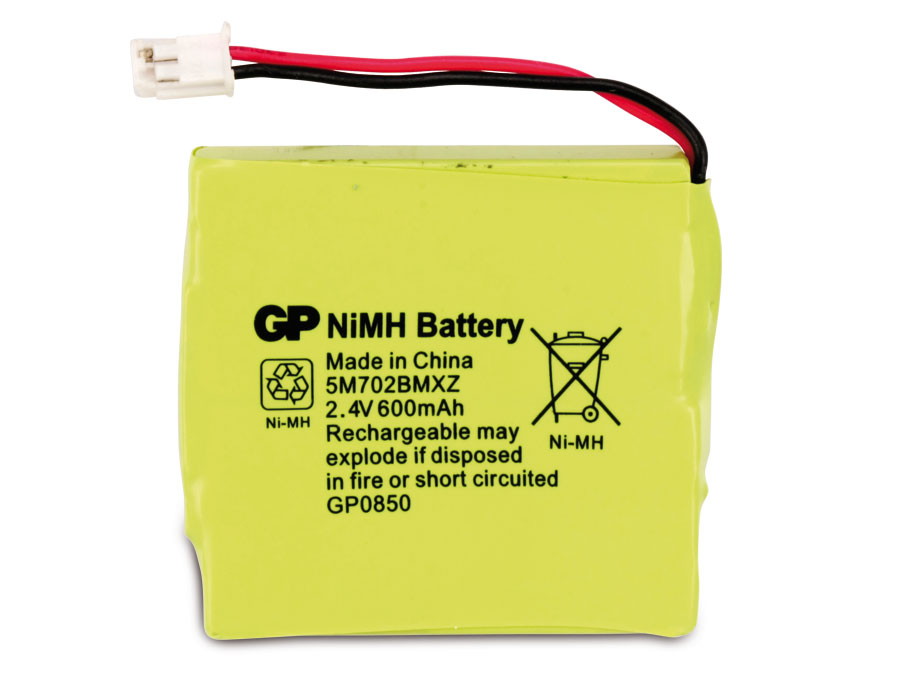
\includegraphics[width=0.5\textwidth]{fig/NiMH.JPG}
\caption{NiMH (Quelle: http://www.pollin.de/shop/index.html)}
\label{fig:Java}
\end{figure}

\begin{table}[h]
\begin{tabular}{p{0.5\textwidth} | p{0.5\textwidth}}


 \textbf{Vorteile} & \textbf{Nachteile} \\ \hline
	 
\begin{itemize}
\item Niedriger Anschaffungspreis für Akku und Ladegerät
\item Relativ unempfindlich in der Handhabung
\item Hohe Energiedichte
\end{itemize}

 
 &
 
\begin{itemize}
\item In der Regel schwerer und grösser als ein LiPo
\end{itemize}

\end{tabular}
\end{table}

\begin{table}[h]
\begin{tabular}{p{0.5\textwidth}p{0.5\textwidth}}


 \textbf{Risiken} & \\ \hline
	 
\begin{itemize}
\item Gewicht und Baugrösse könnte zu Komplikationen bei der Konstruktion des Fahrzeuges führen.
\end{itemize}

 
\end{tabular}
\end{table}

\pagebreak


%##############
\subsection{Lithium-Polymer-Akku}


\begin{figure}[h!]%Position festigen
\centering
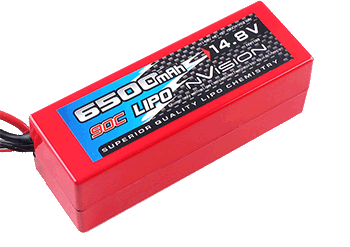
\includegraphics[width=0.5\textwidth]{fig/lipo.png}
\caption{LiPo (Quelle: https://www.cmc-versand.de/)}
\label{fig:Java}
\end{figure}

\begin{table}[h]
\begin{tabular}{p{0.5\textwidth} | p{0.5\textwidth}}


 \textbf{Vorteile} & \textbf{Nachteile} \\ \hline
	 
\begin{itemize}
\item Sehr grosse Auswahl an verschiedenen Bauformen
\item Leicht
\item Sehr hohe Energiedichte
\item Geringe Selbstentladung
\end{itemize}

 
 &
 
\begin{itemize}
\item Hoher Anschaffungspreis für Akku und Ladegerät
\item Empfindlich in der Handhabung
\end{itemize}

\end{tabular}
\end{table}

\begin{table}[h]
\begin{tabular}{p{0.5\textwidth}p{0.5\textwidth}}


 \textbf{Risiken} & \\ \hline
	 
\begin{itemize}
\item Könnte aufgrund der Empfindlichkeit bei nicht fachgerechter Nutzung in der Testphase Schaden nehmen.
\end{itemize}

 
\end{tabular}
\end{table}

\pagebreak